\documentclass[xcolor=svgnames,professionalfonts,11pt,aspectratio=43]{beamer}

%!TEX root = ../thesis.tex

\usepackage[utf8]{inputenc}
\usepackage[T1]{fontenc}
\usepackage[english]{babel}

\usepackage{etoolbox}
\pretocmd{\section}{\clearpage}{}{}

\usepackage{amssymb}

\usepackage{libertine}
\usepackage[scaled=0.83]{beramono}
\usepackage{textcomp}
\usepackage{setspace}
\setlength{\parindent}{0em}
\usepackage[svgnames]{xcolor}
\usepackage{graphicx}
\usepackage{tabularx}

\newcolumntype{b}{>{\bfseries}c}

\usepackage{booktabs}
\usepackage{multirow}

\usepackage{multicol}
\usepackage{lipsum}

\usepackage{listings}
%!TEX root = ../thesis.tex
\definecolor{comment}{HTML}{236E25}
\definecolor{keyword}{HTML}{881280}
\definecolor{ndkeyword}{HTML}{994500}
\definecolor{string}{HTML}{1A1AA6}

\makeatletter
\newcommand{\miniscule}{\@setfontsize\miniscule{5}{6}}% \tiny: 6/7
\makeatother

\lstset{%
  basicstyle=\ttfamily\scriptsize\mdseries\singlespacing,
  %columns=fullflexible,
  breakatwhitespace=false,
  breaklines=true,
  numbers=left,
  numberstyle=\ttfamily\scriptsize,
  stepnumber=5,
  numberfirstline=false,
  firstnumber=1,
  showstringspaces=false,
  tabsize=2,
  backgroundcolor=\color{white},
  captionpos=t,
  frame=L,
  float=htb,
  xleftmargin=\bigskipamount,
  xrightmargin=\bigskipamount,
  aboveskip=\bigskipamount,
  belowskip=\bigskipamount,
  commentstyle=\color{comment},
  stringstyle=\color{string},
  identifierstyle=\color{black},
  keywordstyle=\color{keyword}\bfseries,
  ndkeywordstyle=\color{ndkeyword},
}

\lstset{literate=
  {á}{{\'a}}1 {é}{{\'e}}1 {í}{{\'i}}1 {ó}{{\'o}}1 {ú}{{\'u}}1
  {Á}{{\'A}}1 {É}{{\'E}}1 {Í}{{\'I}}1 {Ó}{{\'O}}1 {Ú}{{\'U}}1
  {à}{{\`a}}1 {è}{{\'e}}1 {ì}{{\`i}}1 {ò}{{\`o}}1 {ù}{{\`u}}1
  {À}{{\`A}}1 {È}{{\'E}}1 {Ì}{{\`I}}1 {Ò}{{\`O}}1 {Ù}{{\`U}}1
  {ä}{{\"a}}1 {ë}{{\"e}}1 {ï}{{\"i}}1 {ö}{{\"o}}1 {ü}{{\"u}}1
  {Ä}{{\"A}}1 {Ë}{{\"E}}1 {Ï}{{\"I}}1 {Ö}{{\"O}}1 {Ü}{{\"U}}1
  {â}{{\^a}}1 {ê}{{\^e}}1 {î}{{\^i}}1 {ô}{{\^o}}1 {û}{{\^u}}1
  {Â}{{\^A}}1 {Ê}{{\^E}}1 {Î}{{\^I}}1 {Ô}{{\^O}}1 {Û}{{\^U}}1
  {œ}{{\oe}}1 {Œ}{{\OE}}1 {æ}{{\ae}}1 {Æ}{{\AE}}1 {ß}{{\ss}}1
  {ç}{{\c c}}1 {Ç}{{\c C}}1 {ø}{{\o}}1 {å}{{\r a}}1 {Å}{{\r A}}1
  {€}{{\EUR}}1 {£}{{\pounds}}1 {°}{{\textdegree}}1
  {µ}{{$\mathrm{\mu}$}}1
  {±}{{$\pm$}}1
  {σ}{{$\mathrm{\sigma}$}}1
  {⋅}{{$\cdot$}}1
}
\lstdefinelanguage{JavaScript}{
  morekeywords={break, case, catch, continue, debugger, default, delete, do, else, finally, for, function, if, in, instanceof, new, return, switch, this, throw, try, typeof, var, while, with, null, throw, this},
  morendkeywords={Object,Array,Boolean,Date,window,Number,String,Math,XMLHttpRequest,document,prototype,undefined,Infinity,NaN,import,export,this,console,Error},
  sensitive,
  comment=[l]{//},
  morecomment=[s]{/*}{*/},
  morestring=[b]',
  morestring=[b]",
}
\lstdefinelanguage{XML}{
  morestring=[b]",
  morecomment=[s]{<?}{?>},
  morecomment=[s]{<!--}{-->},
  morecomment=[s]{&}{;},
  alsoletter={:},
  morekeywords={
    ComplexData,
    ComplexOutput,
    DataInputs,
    Default,
    Encoding,
    Format,
    hello,% remove,
    Input,
    LiteralData,
    LiteralOutput,
    MimeType,
    Output,
    ows:Abstract,
    ows:AnyValue,
    ows:DataType,
    ows:Identifier,
    ows:LowerCorner,
    ows:Title,
    ows:UOM,
    UOMs,
    ows:UpperCorner,
    ProcessDescription,
    ProcessOutputs,
    soap:Body,
    soap:Envelope,
    soap:Header,
    stream:InputMessage,
    stream:Inputs,
    stream:Output,
    stream:OutputMessage,
    stream:OutputRequestMessage,
    stream:Outputs,
    stream:ProcessID,
    ows:AllowedValues,
    ows:Value,
    stream:Reference,
    stream:ReferenceInput,
    stream:StopMessage,
    stream:StreamingInput,
    Supported,
    wps:BoundingBoxData,
    wps:ComplexData,
    wps:Data,
    wps:DataInputs,
    wps:Execute,
    wps:ExecuteResponse,
    wps:Input,
    wps:LiteralData,
    wps:Output,
    wps:Process,
    wps:ProcessDescriptions,
    wps:ProcessOutputs,
    wps:ProcessSucceeded,
    wps:Reference,
    wps:Status,
    wsa:Action,
    wsa:Address,
    wsa:FaultTo,
    wsa:From,
    wsa:MessageID,
    wsa:RelatesTo,
    wsa:ReplyTo,
    wsa:To,
  },
  morendkeywords={
    creationTime,
    crs,
    dataType,
    dimensions,
    encoding,
    includeInputs,
    maxOccurs,
    method,
    mimeType,
    minOccurs,
    ows:reference,
    RelationshipType,
    service,
    serviceInstance,
    statusSupported,
    storeSupported,
    version,
    wps:processVersion,
    xlink:href,
    xml:lang,
    xmlns:ows,
    xmlns:soap,
    xmlns:stream,
    xmlns:wps,
    xmlns:wsa,
    xmlns:xlink,
  }
}
\newcommand{\texttag}[2]{\texttt{\tiny{\textless\textcolor{keyword}{#1:#2}\textgreater}}}
\newcommand{\includecode}[2][xml]{\lstinputlisting[]}

\usepackage{enumitem}
\setlist{nolistsep}

\usepackage[hyphens]{url}
\urlstyle{same}
\renewcommand{\UrlBreaks}{%
\do\a\do\b\do\c\do\d\do\e\do\f%
\do\g\do\h\do\i\do\j\do\k\do\l%
\do\m\do\n\do\o\do\p\do\q\do\r%
\do\u\do\v\do\w\do\x\do\y\do\z%
\do\A\do\B\do\C\do\D\do\E\do\F%
\do\G\do\H\do\I\do\J\do\K\do\L%
\do\M\do\N\do\O\do\P\do\Q\do\R%
\do\U\do\V\do\W\do\X\do\Y\do\Z%
\do\_\do\/\do\-}

%\usepackage{titlesec}
%\titleformat{\paragraph}[hang]{\sffamily\bfseries}{\theparagraph}{.5em}{}
%\titleformat{\subparagraph}[hang]{\sffamily\bfseries}{\thesubparagraph}{.5em}{}

\usepackage[unicode,breaklinks,hidelinks,colorlinks=true,urlcolor=black,linkcolor=black,citecolor=black]{hyperref}

\usepackage[authoryear,round,comma,sort&compress]{natbib}

\usepackage[margin=10pt,labelfont={bf},format=plain]{caption}

\bibliographystyle{plainnat}

\usepackage{acronym}
%!TEX root = ../thesis.tex

\acrodef{WPS}{Web Processing Service}
\acrodef{OGC}{Open Geospatial Consortium}
\acrodef{DAG}{Directed Acyclic Graph}
\acrodef{BFS}{Breadth-first search}

\usepackage{listings}

\hypersetup{
    pdftitle={Streaming Web-Services for Calculating Live Hydrological Derivatives},
    pdfsubject={Master Thesis},
    pdfauthor={Christian Autermann}
}

\newcommand{\fu}[1]{\footnote{\url{#1}}}
\newcommand{\mail}[1]{\href{mailto:#1}{#1}}



\newsavebox\mybox
\newenvironment{signedquote}[1]
  {\savebox\mybox{\small\textup{--- #1}}\begin{quote}\itshape}
  {{\leavevmode\unskip\nobreak\hfil\penalty50\hskip2em
  	\hbox{}\nobreak\hfil\usebox\mybox\parfillskip=0pt
    \finalhyphendemerits=0\endgraf}\end{quote}}

\title{Streaming Web-Services for Calculating Live Hydrological Derivatives}
\subtitle{Master Thesis Defense}
\institute{Supervisors: Edzer Pebesma (IfGI), Jordan Read (USGS CIDA)}
\author{Christian Autermann}
\date{January 31, 2014}

\begin{document}

\frame{\titlepage}

\begin{frame}[t]{Outline}
  \begin{enumerate}
    \item Lake Analyzer
    \item Matlab WPS
    \item Lake Analyzer WPS
    \item Streaming WPS
    \item Current Status
  \end{enumerate}
\end{frame}

\titleframe{Lake Analyzer}

\begin{frame}[t]{Lake Analyzer}
  \begin{itemize}
    \item Developed at University of Wisconsin/USGS
    \item Analysis of high-frequency lake buoys data
    \item Written in Matlab (R version with less features exist)
    \pause
    \item[]
    \begin{columns}
    \column{.45\textwidth}
      \begin{itemize}
        \arrow Wind speed
        \arrow Water temperature
        \arrow Schmidt stability
        \arrow (Parent) buoyancy frequency
        \arrow (Parent) lake number
        \arrow (Parent) Mode one vertical seiche period
      \end{itemize}
      \column{.45\textwidth}
      \begin{itemize}
        \arrow (Parent) metalimnion bottom depth
        \arrow (Parent) metalimnion top depth
        \arrow (Parent) thermocline depth
        \arrow (Parent) u star (turblent velocity scale from wind)
        \arrow (Parent) Wedderburn number
      \end{itemize}
    \end{columns}
  \end{itemize}
\end{frame}

\begin{frame}[c,fragile]{Lake Analyzer}
  \begin{figure}
    \centering
    \subfigure{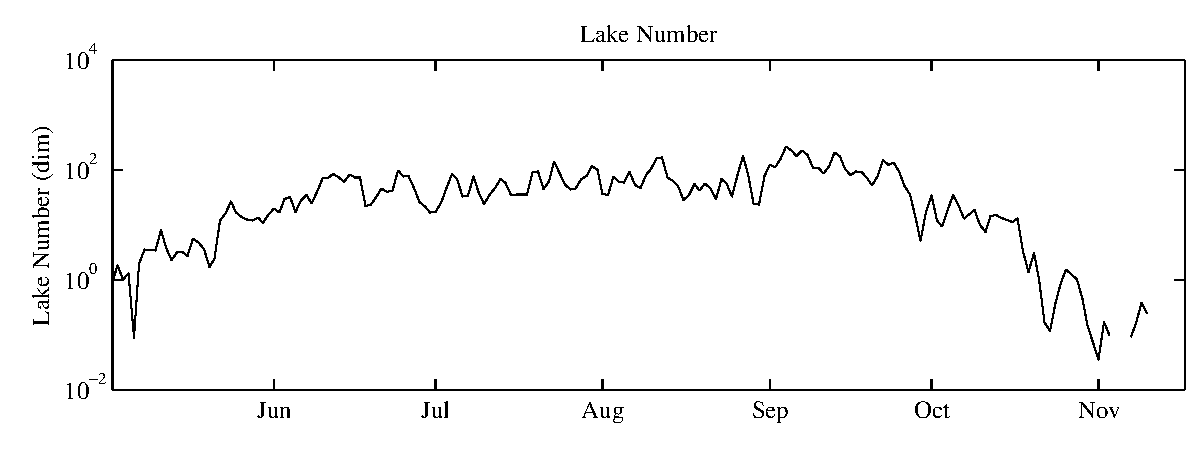
\includegraphics[width=.25\textwidth]{figures/Sparkling_Ln.pdf}}
    \subfigure{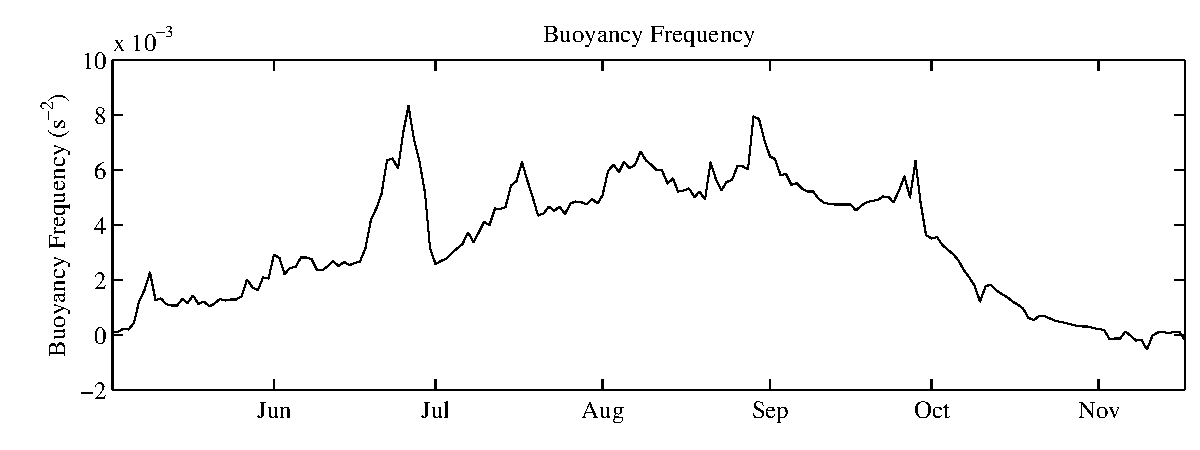
\includegraphics[width=.25\textwidth]{figures/Sparkling_N2.pdf}}
    \subfigure{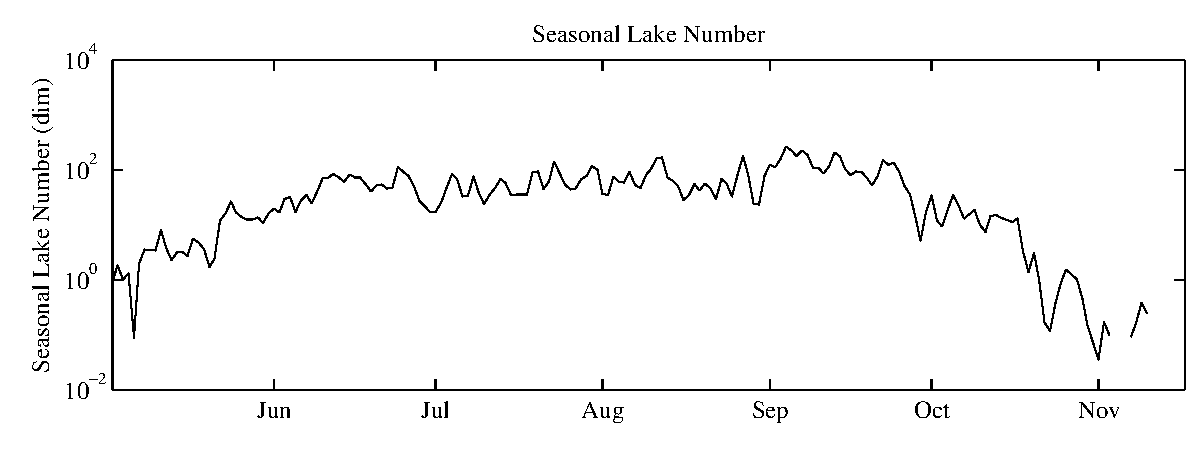
\includegraphics[width=.25\textwidth]{figures/Sparkling_SLn.pdf}}\\
    \subfigure{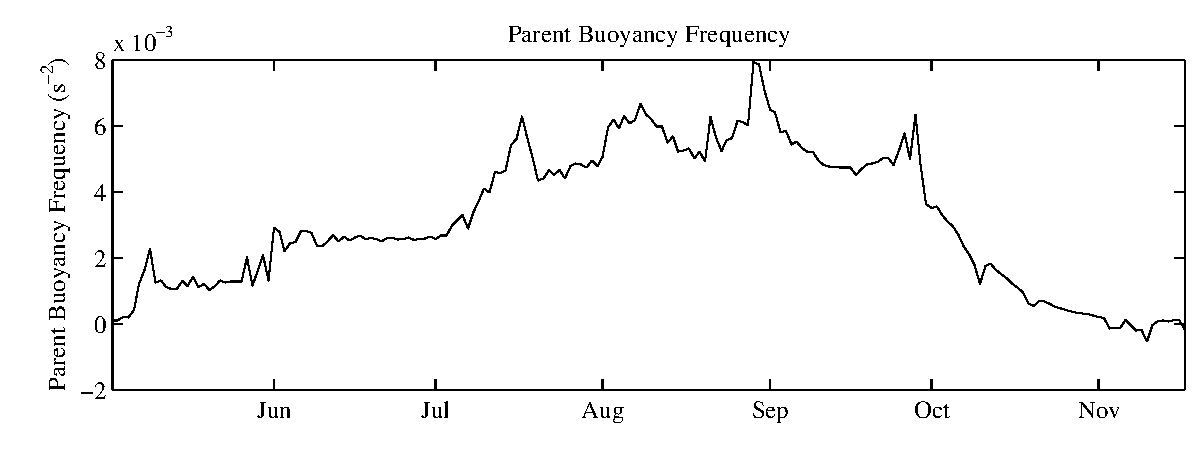
\includegraphics[width=.25\textwidth]{figures/Sparkling_SN2.pdf}}
    \subfigure{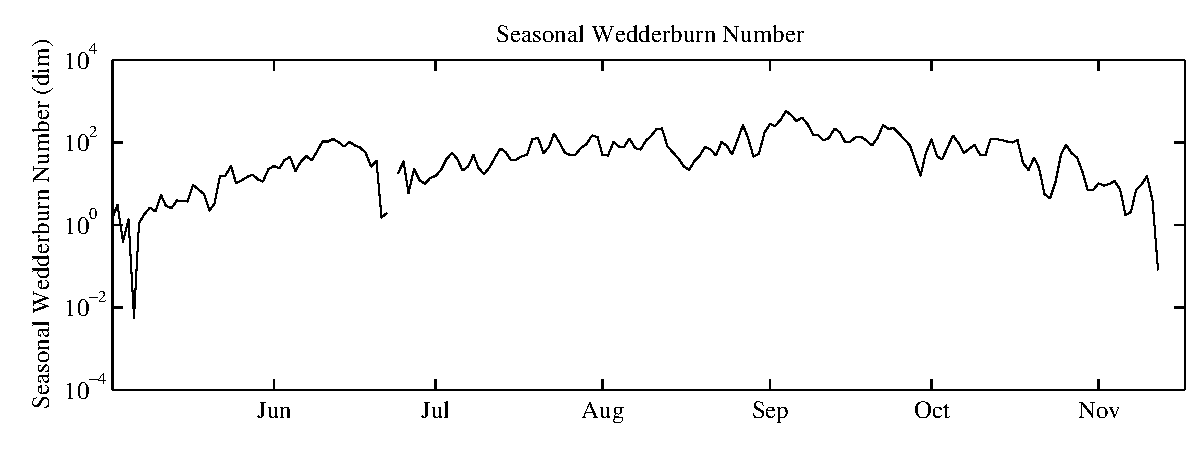
\includegraphics[width=.25\textwidth]{figures/Sparkling_SW.pdf}}
    \subfigure{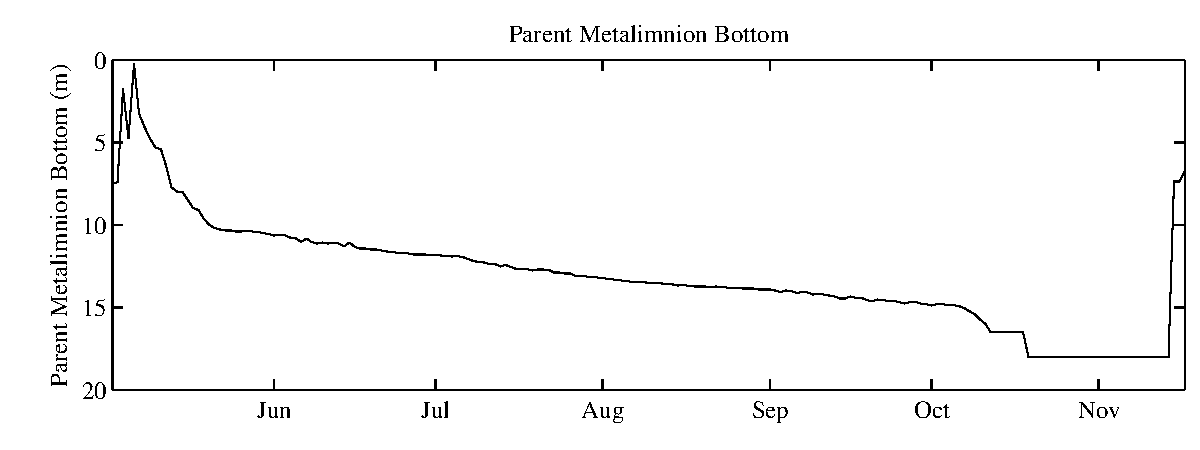
\includegraphics[width=.25\textwidth]{figures/Sparkling_SmetaB.pdf}}\\
    \subfigure{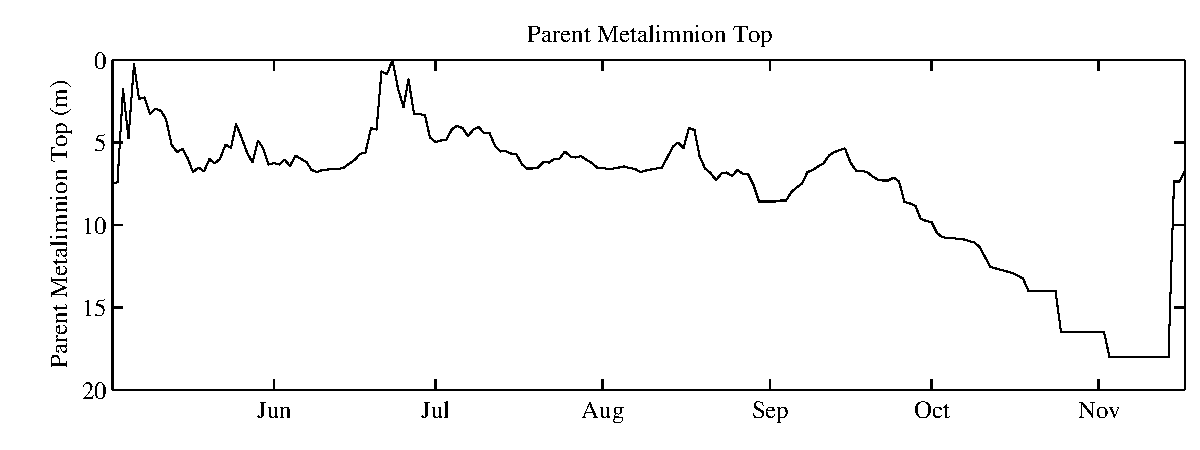
\includegraphics[width=.25\textwidth]{figures/Sparkling_SmetaT.pdf}}
    \subfigure{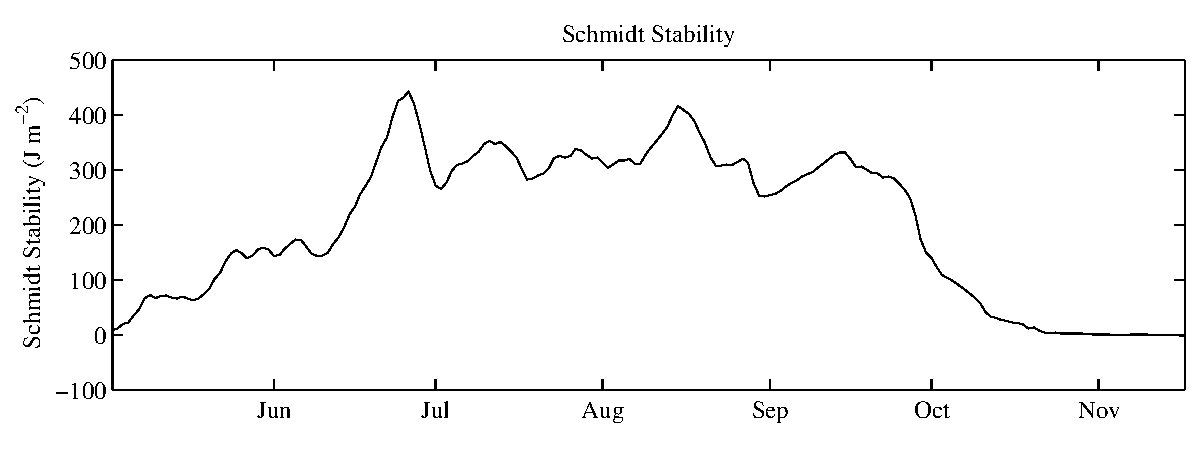
\includegraphics[width=.25\textwidth]{figures/Sparkling_St.pdf}}
    \subfigure{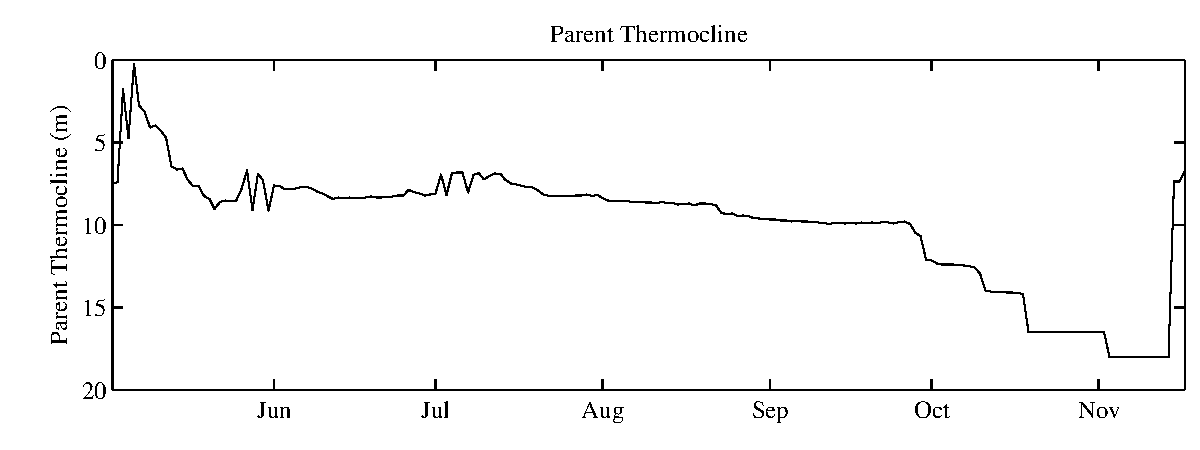
\includegraphics[width=.25\textwidth]{figures/Sparkling_SthermD.pdf}}\\
    \subfigure{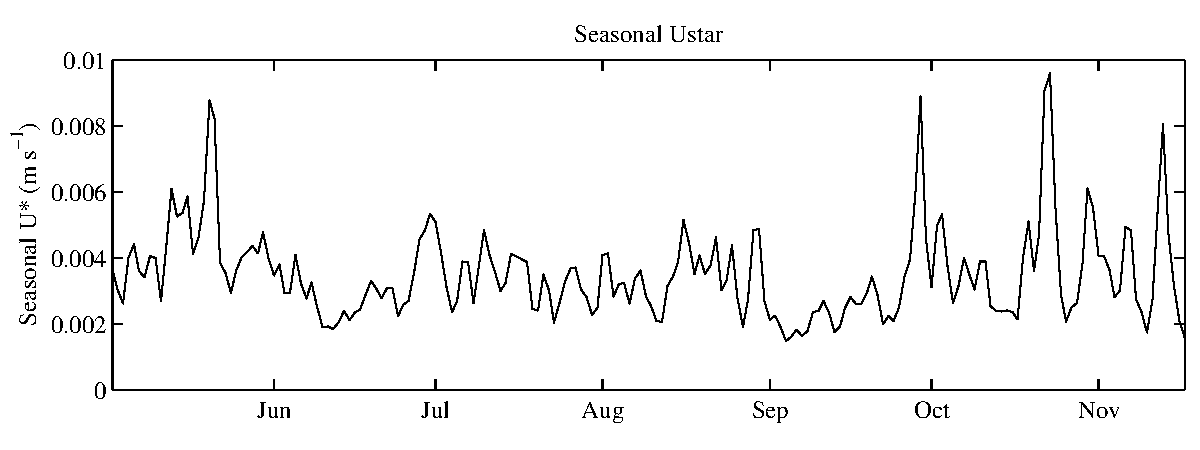
\includegraphics[width=.25\textwidth]{figures/Sparkling_SuSt.pdf}}
    \subfigure{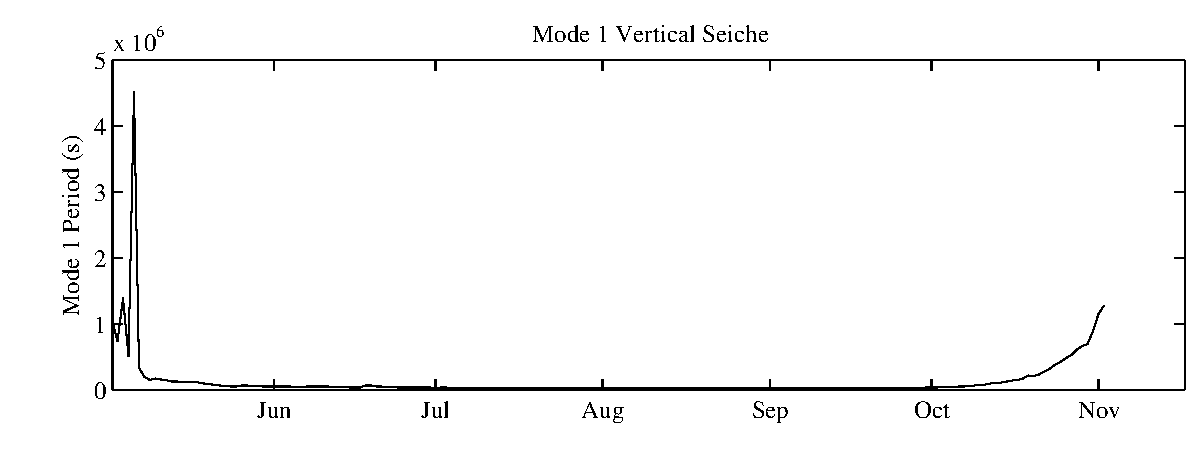
\includegraphics[width=.25\textwidth]{figures/Sparkling_T1.pdf}}
    \subfigure{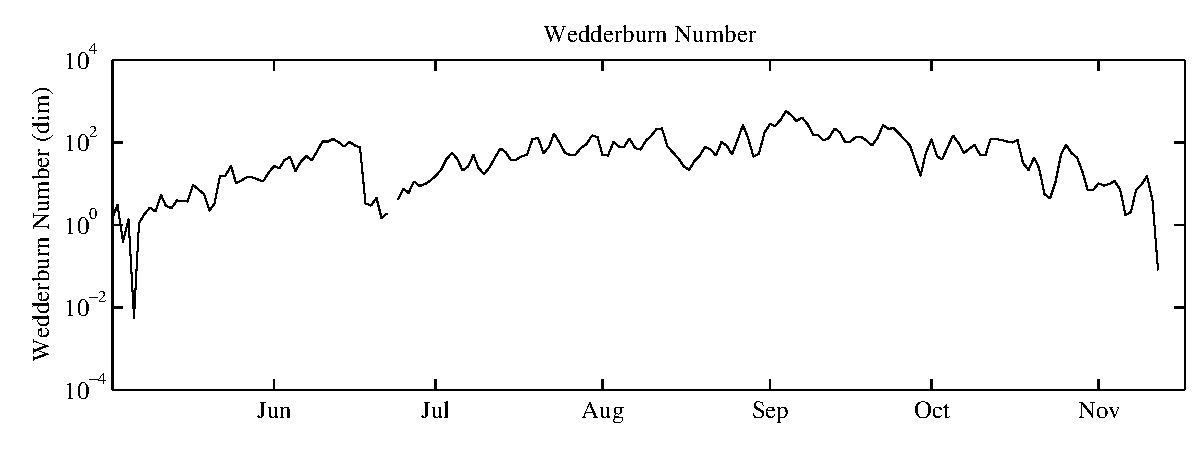
\includegraphics[width=.25\textwidth]{figures/Sparkling_W.pdf}}\\
    \subfigure{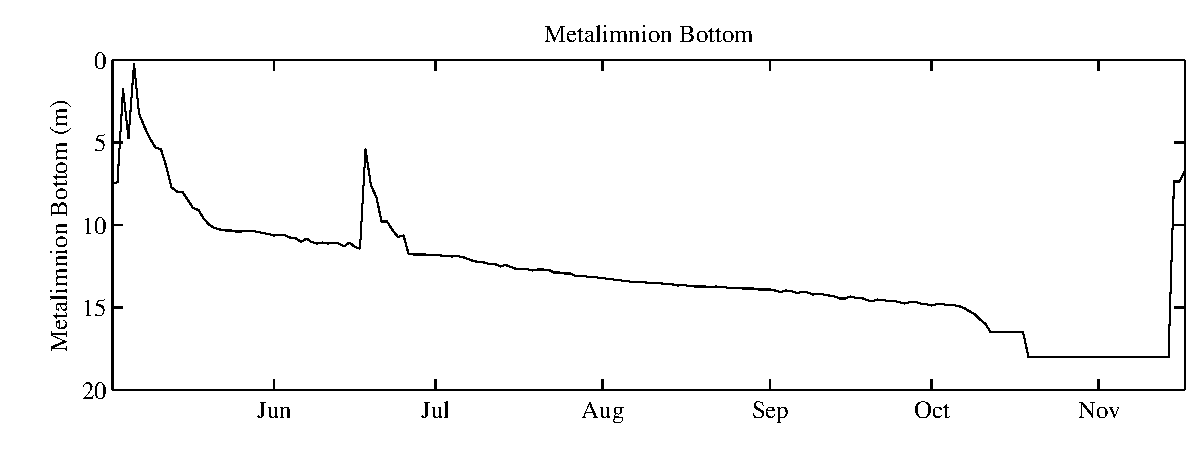
\includegraphics[width=.25\textwidth]{figures/Sparkling_metaB.pdf}}
    \subfigure{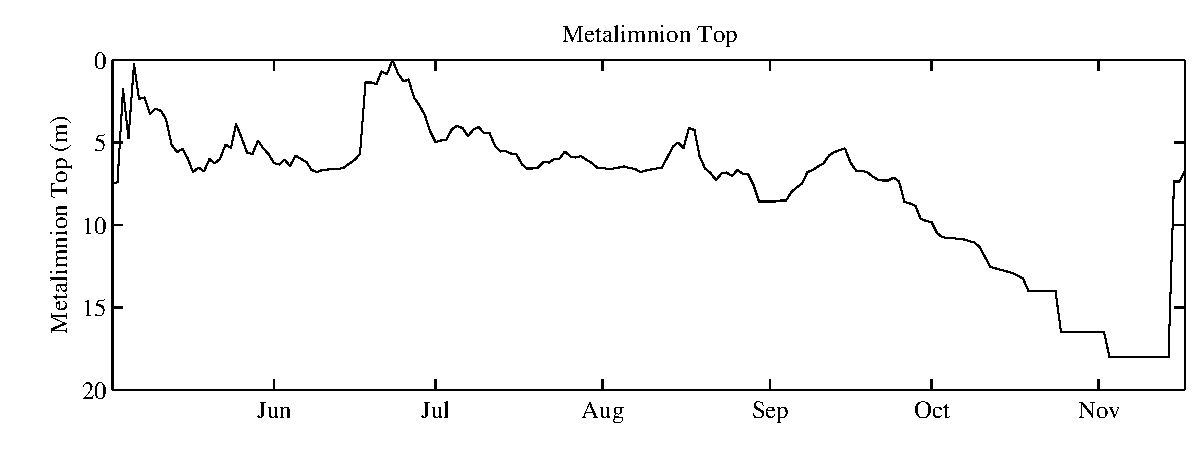
\includegraphics[width=.25\textwidth]{figures/Sparkling_metaT.pdf}}
    \subfigure{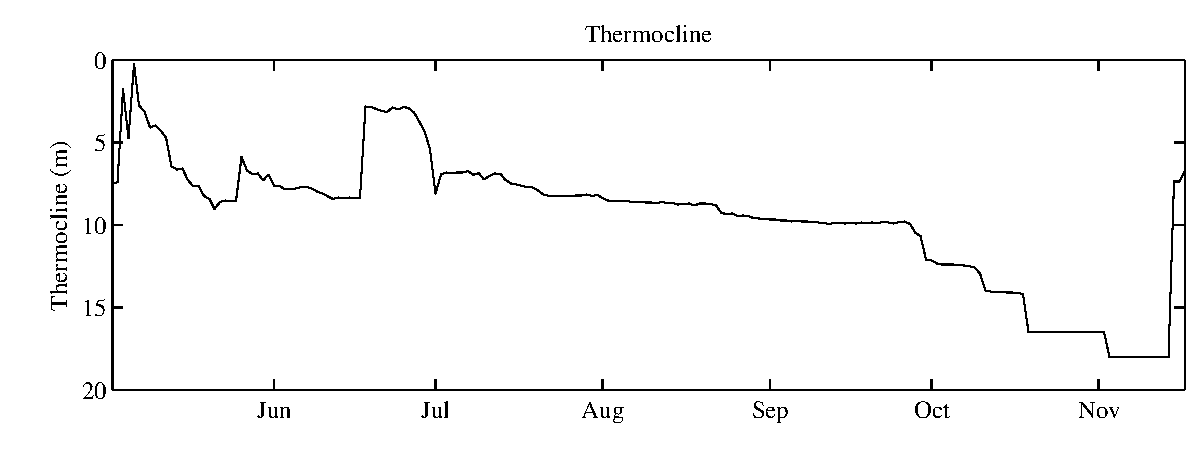
\includegraphics[width=.25\textwidth]{figures/Sparkling_thermD.pdf}}\\
    \subfigure{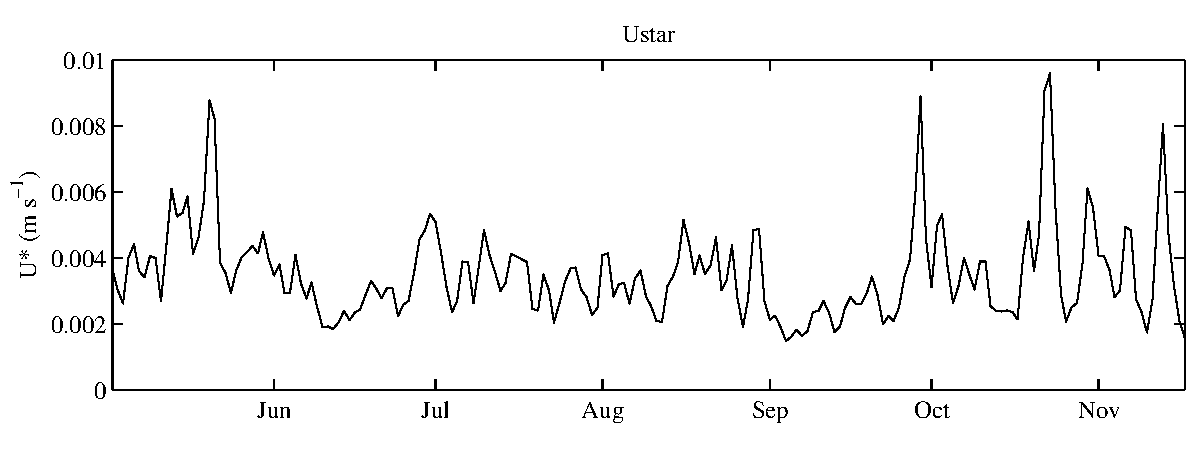
\includegraphics[width=.25\textwidth]{figures/Sparkling_uSt.pdf}}
    \subfigure{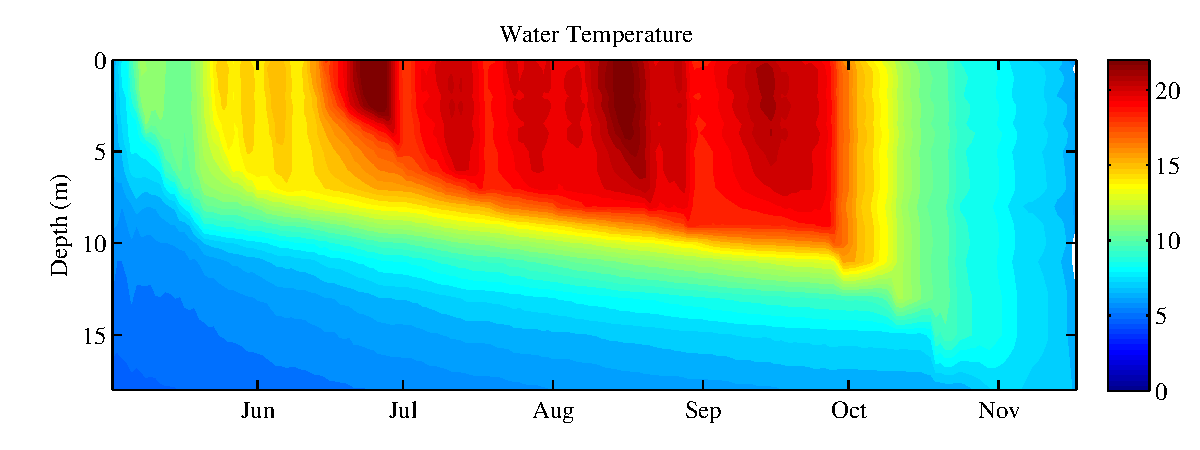
\includegraphics[width=.25\textwidth]{figures/Sparkling_wTemp.pdf}}
    \subfigure{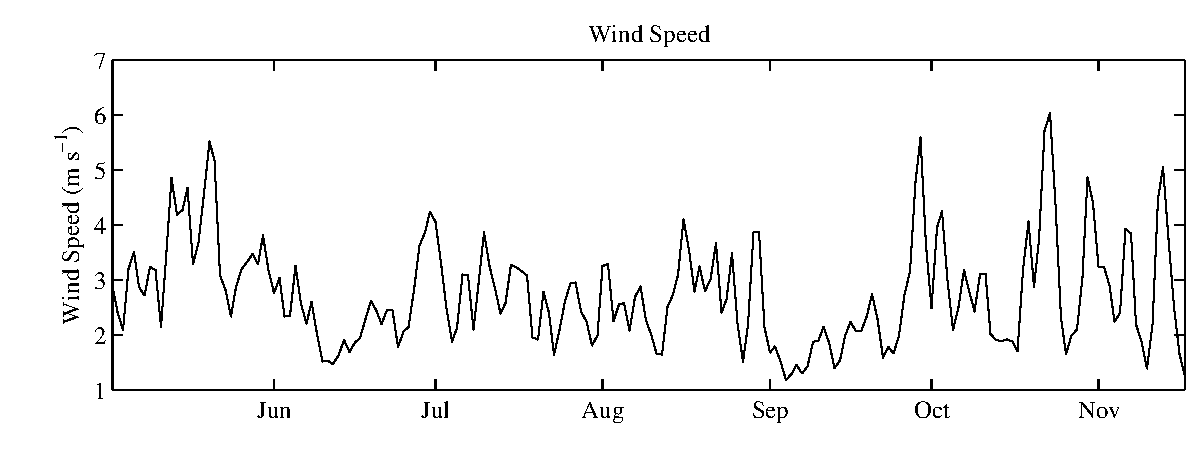
\includegraphics[width=.25\textwidth]{figures/Sparkling_wndSpd.pdf}}
  \end{figure}
\end{frame}

\begin{frame}[c]{Lake Analyzer}
  \begin{itemize}
    \item How to to integreate Lake Analyzer into web-processing chains?
    \pause
    \item How to offer live analysis of real-time data?
    \pause
    \item How to analyze hundreds, thousands, or millions of lakes?
  \end{itemize}
\end{frame}

\titleframe{Matlab WPS}

\begin{frame}[t]{Matlab WPS}
  \begin{itemize}
    \item Offering Matlab functions as WPS processes
    \item Implemented as a 52\textdegree{}N WPS backend (and standalone version)
    \item Configuration with simple YAML file
    \item Similar approach to WPS4R, but\dots
    \begin{itemize}
      \item uses seperated configuration file for each script
      \item complex inputs/outputs are handled in Matlab
      \pause
      \arrow tradeoff: no output conversion between different formats
    \end{itemize}
  \end{itemize}
\end{frame}

\begin{frame}[fragile]{Matlab WPS --- Example}
  \begin{columns}
    \column{.39\textwidth}
    \lstinputlisting[language=Matlab]{listings/matlab-add-function.m}
    \pause
    \lstinputlisting{listings/matlab-add-process-configuration.yaml}
    \pause
    \column{.61\textwidth}
    \lstinputlisting[language=XML]{listings/matlab-add-process-description.xml}
  \end{columns}
\end{frame}

\begin{frame}[c,fragile]{Matlab WPS --- Accessing Matlab from the Web}
  \begin{columns}
    \column{.37\textwidth}
    \lstinputlisting[language=Matlab]{listings/matlab-add-function.m}
    \pause
    \lstinputlisting{listings/matlab-connector.sh}
    \pause
    \column{.63\textwidth}
    \lstinputlisting[language=JavaScript]{listings/matlab-add-javascript-client.js}
  \end{columns}
\end{frame}

%\begin{frame}[t]{Matlab WPS --- Accessing Matlab from the Web}
%  \begin{itemize}
%    \item Matlab is proprietary and commercial software
%    \pause
%    \item Accessing Matlab in this manner only allowed \dots
%    \begin{itemize}
%      \item for the \emph{Network Concurrent User Activation Type}
%      \pause
%      \item for the \emph{Standalone Named User Activation Type}
%      \item for the \emph{Network Named User Activation Type}
%    \end{itemize}
%  \end{itemize}
%\end{frame}

\begin{frame}[c,fragile]{Matlab WPS --- Websockets}
  \begin{columns}
    \column{.45\textwidth}
    \lstinputlisting{listings/websocket-handshake-request.txt}
    \pause
    \column{.45\textwidth}
    \lstinputlisting{listings/websocket-handshake-response.txt}
  \end{columns}
  \pause
  \begin{columns}
  \column{.45\textwidth}
  Full-Duplex TCP connection
  \pause
  \column{.45\textwidth}
  Widely supported:
  \begin{itemize}
    \item IE \textgreater10
    \item Firefox \textgreater6
    \item Chrome \textgreater14
    \item Safari \textgreater6
    \item Opera \textgreater12.1
  \end{itemize}
  \end{columns}
\end{frame}

\titleframe{Lake Analyzer WPS}

\begin{frame}[t]{Lake Analyzer WPS}
  \begin{itemize}
    \item simple implementation using the \emph{Matlab WPS}
    \item small modifications to the script to allow file transfers
    \item wrapper function to get rid of configuration files
  \end{itemize}
\end{frame}

\begin{frame}[c,fragile]{Lake Analyzer WPS --- Wrapper Function}
    \begin{center}
      \lstinputlisting[language=Matlab,lastline=10]{listings/lake-analyzer-wps-wrapper.m}
    \end{center}
\end{frame}

\begin{frame}[c,fragile]{Lake Analyzer WPS --- Configuration}
    \begin{center}
      \lstinputlisting[lastline=40]{listings/lake-analyzer-wps-configuration.yaml}
    \end{center}
\end{frame}

\begin{frame}[c,fragile]{Lake Analyzer WPS --- Process Description}
    \begin{center}
      \lstinputlisting[language=XML,lastline=40]{listings/lake-analyzer-wps-process-description.xml}
    \end{center}
\end{frame}

\begin{frame}[c,fragile]{Lake Analyzer WPS --- Process Description}
    \begin{center}
      \lstinputlisting[language=XML,firstline=451,lastline=484]{listings/lake-analyzer-wps-process-description.xml}
    \end{center}
\end{frame}

\begin{frame}[c,fragile]{Lake Analyzer WPS --- Example Request}
    \begin{center}
      \lstinputlisting[language=XML,lastline=40]{listings/lake-analyzer-wps-request.xml}
    \end{center}
\end{frame}

\begin{frame}[c,fragile]{Lake Analyzer WPS --- Example Response}
    \begin{center}
      \lstinputlisting[language=XML,lastline=20]{listings/lake-analyzer-wps-response.xml}
    \end{center}
\end{frame}

\begin{frame}[c,fragile]{Lake Analyzer WPS --- Example Response}
    \begin{center}
      \lstinputlisting[language=XML,firstline=426,lastline=490]{listings/lake-analyzer-wps-response.xml}
    \end{center}
\end{frame}

\begin{frame}[c,fragile]{Lake Analyzer WPS --- Example Response}
  \begin{figure}
    \centering
    \subfigure{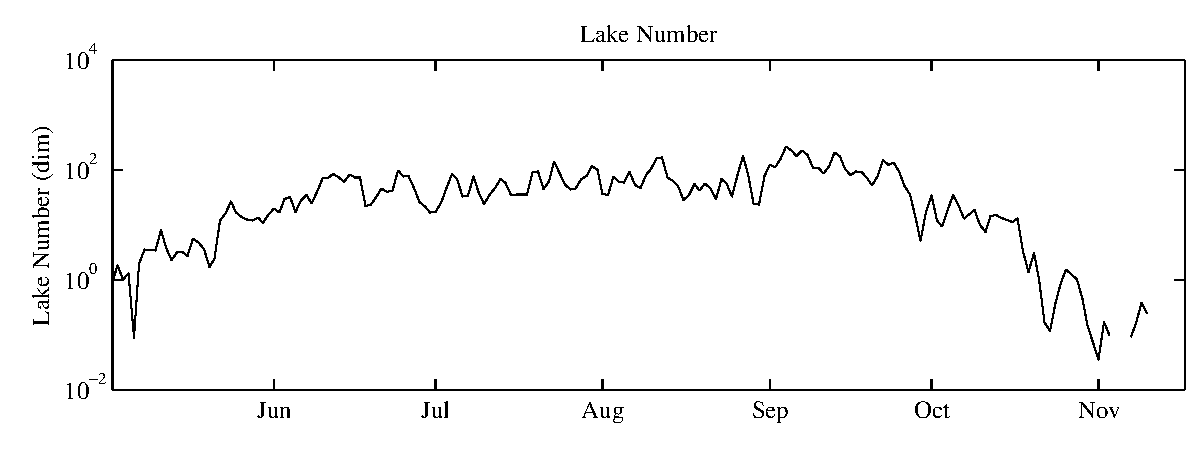
\includegraphics[width=.25\textwidth]{figures/Sparkling_Ln.pdf}}
    \subfigure{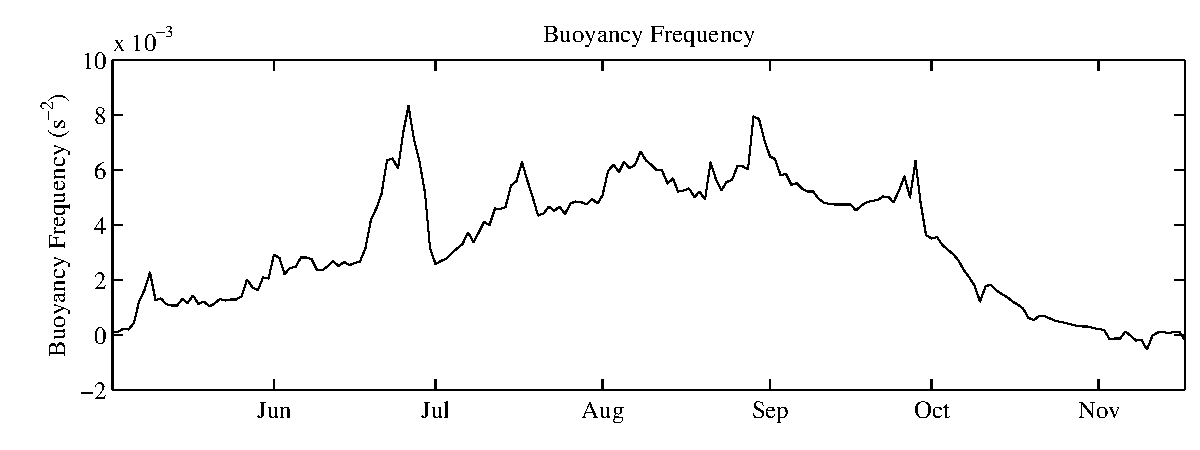
\includegraphics[width=.25\textwidth]{figures/Sparkling_N2.pdf}}
    \subfigure{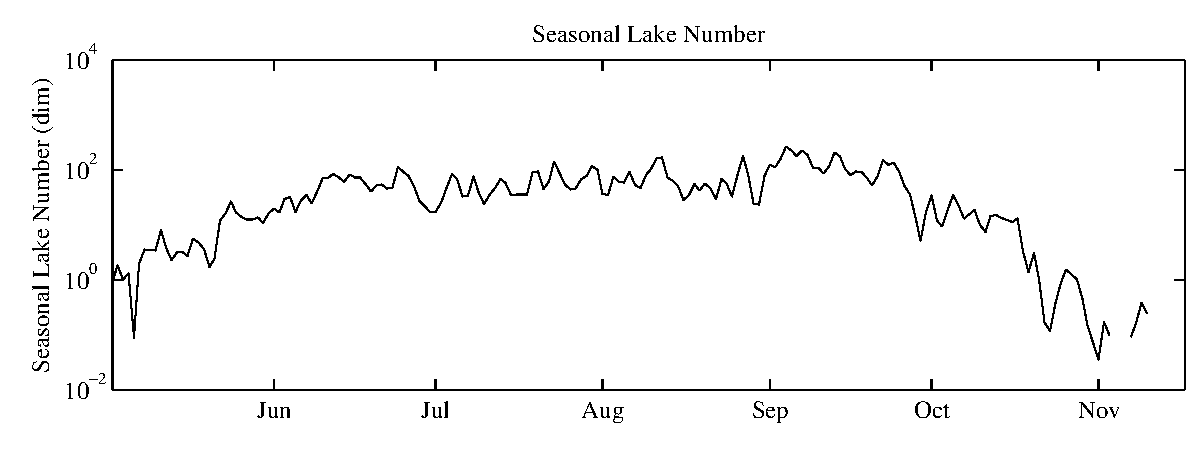
\includegraphics[width=.25\textwidth]{figures/Sparkling_SLn.pdf}}\\
    \subfigure{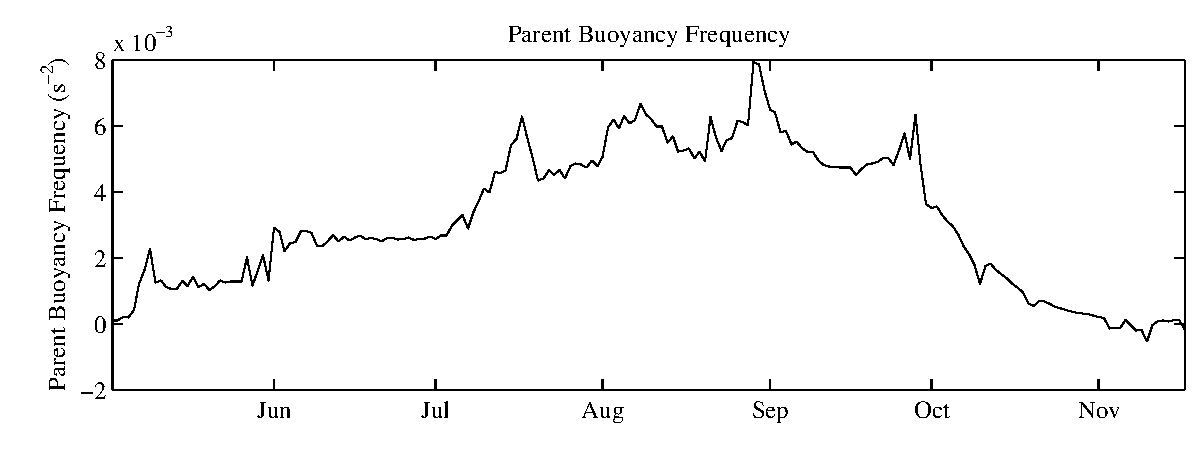
\includegraphics[width=.25\textwidth]{figures/Sparkling_SN2.pdf}}
    \subfigure{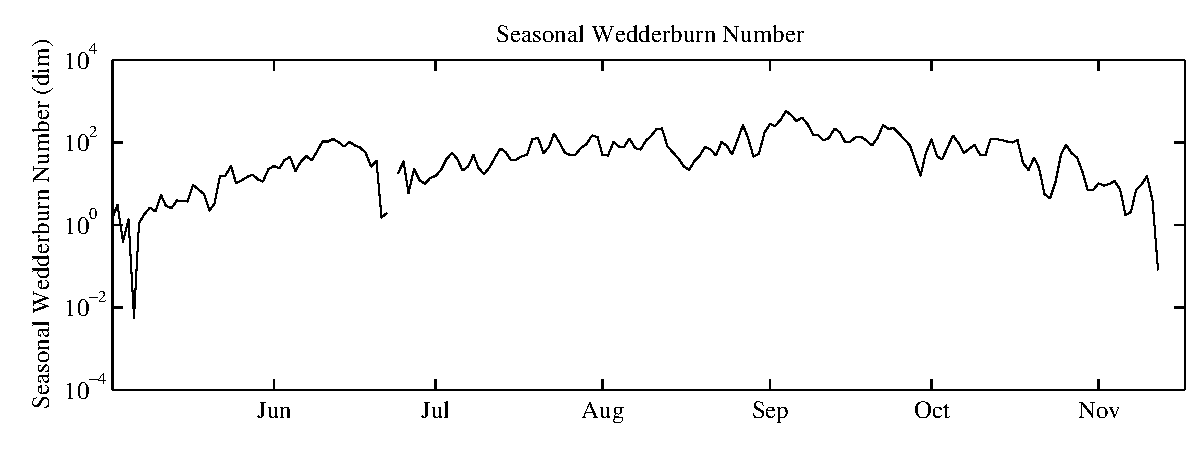
\includegraphics[width=.25\textwidth]{figures/Sparkling_SW.pdf}}
    \subfigure{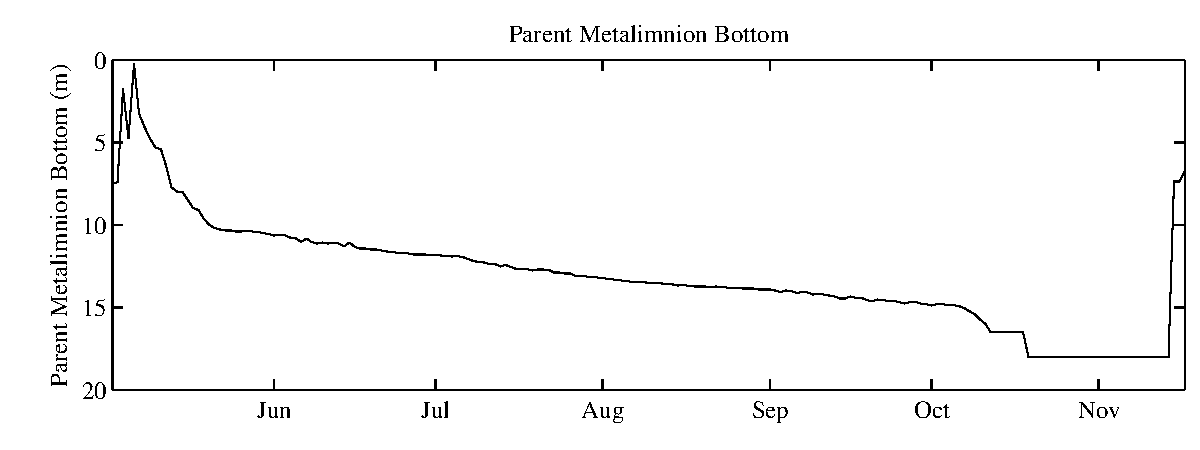
\includegraphics[width=.25\textwidth]{figures/Sparkling_SmetaB.pdf}}\\
    \subfigure{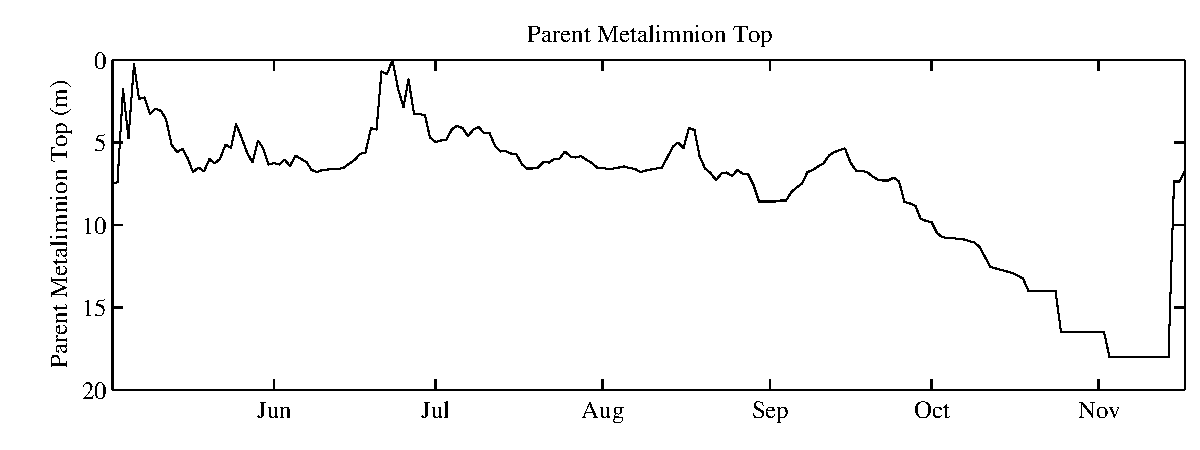
\includegraphics[width=.25\textwidth]{figures/Sparkling_SmetaT.pdf}}
    \subfigure{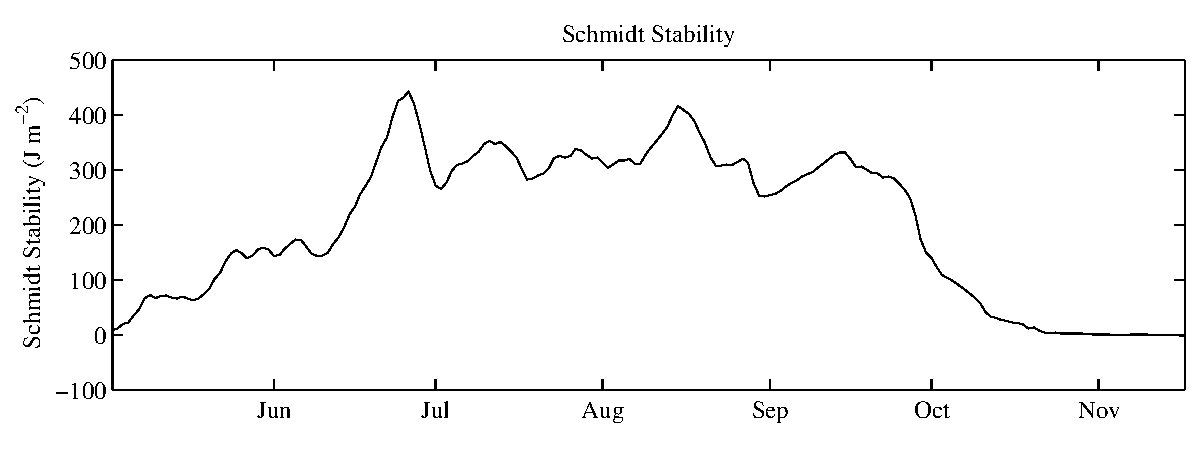
\includegraphics[width=.25\textwidth]{figures/Sparkling_St.pdf}}
    \subfigure{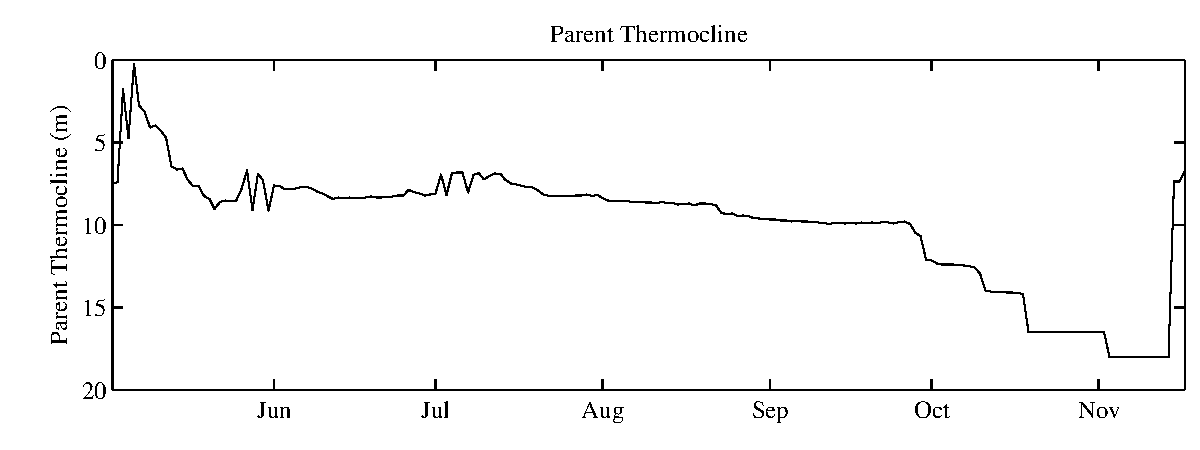
\includegraphics[width=.25\textwidth]{figures/Sparkling_SthermD.pdf}}\\
    \subfigure{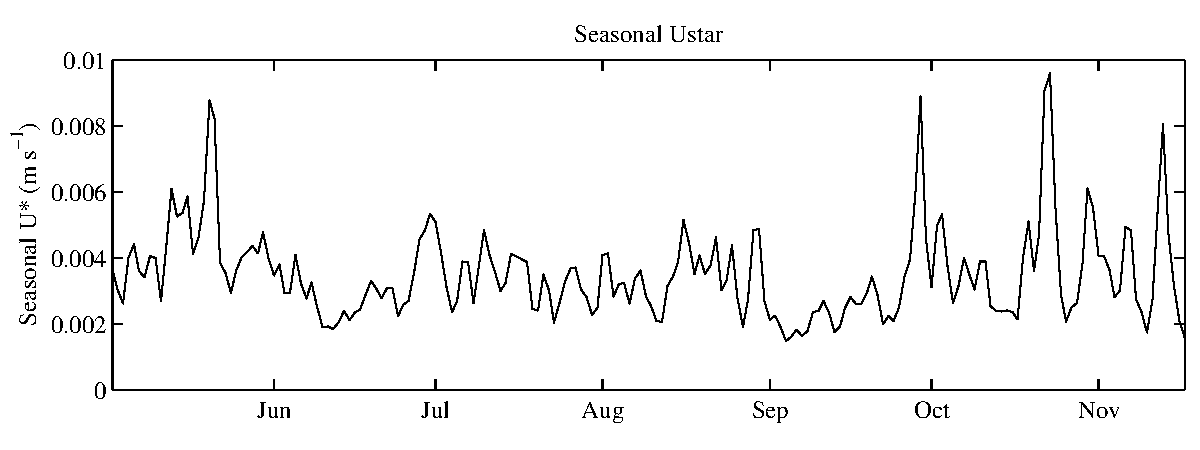
\includegraphics[width=.25\textwidth]{figures/Sparkling_SuSt.pdf}}
    \subfigure{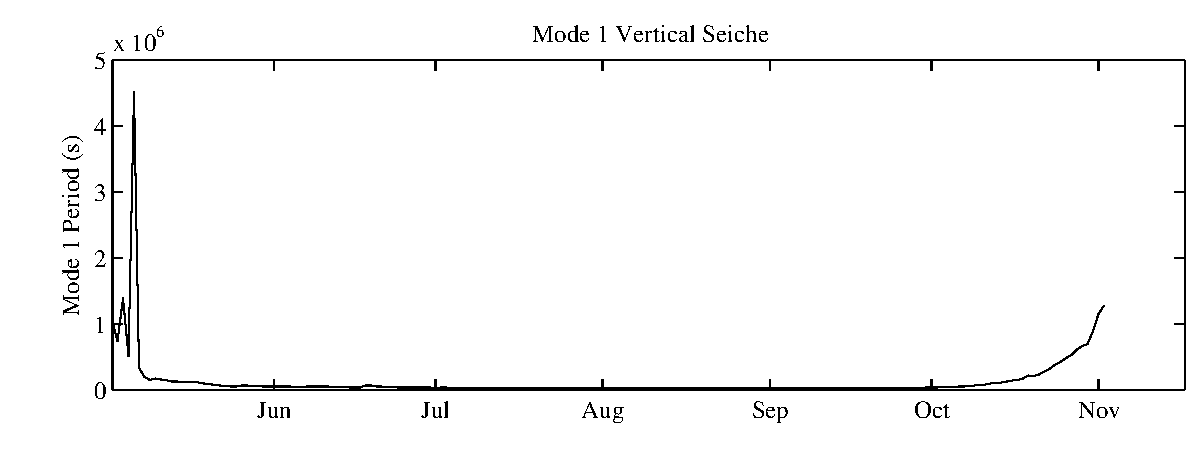
\includegraphics[width=.25\textwidth]{figures/Sparkling_T1.pdf}}
    \subfigure{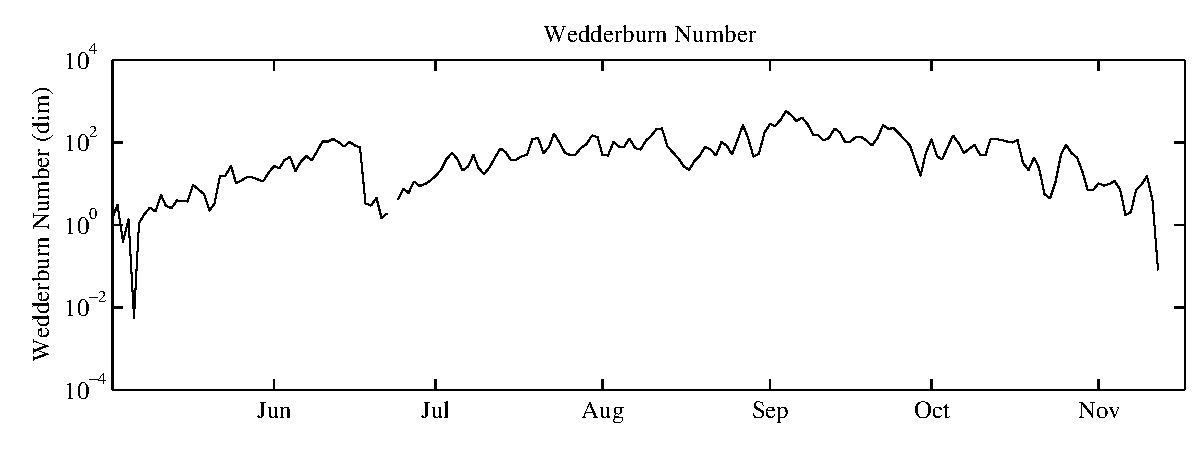
\includegraphics[width=.25\textwidth]{figures/Sparkling_W.pdf}}\\
    \subfigure{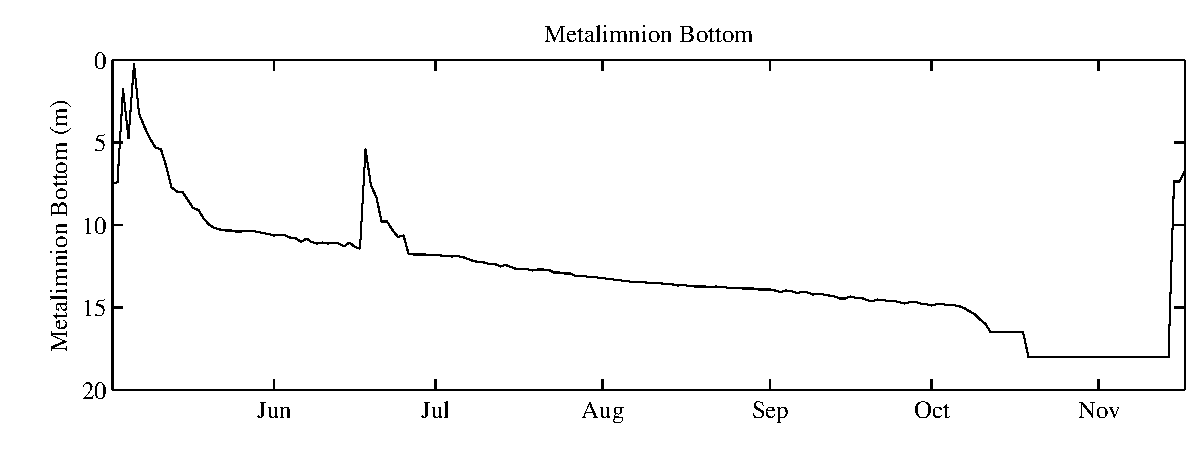
\includegraphics[width=.25\textwidth]{figures/Sparkling_metaB.pdf}}
    \subfigure{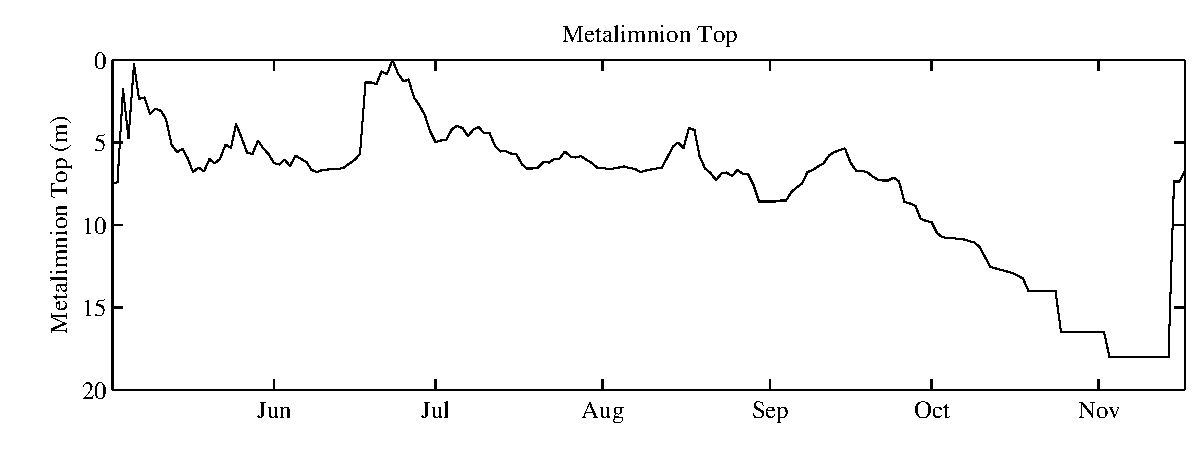
\includegraphics[width=.25\textwidth]{figures/Sparkling_metaT.pdf}}
    \subfigure{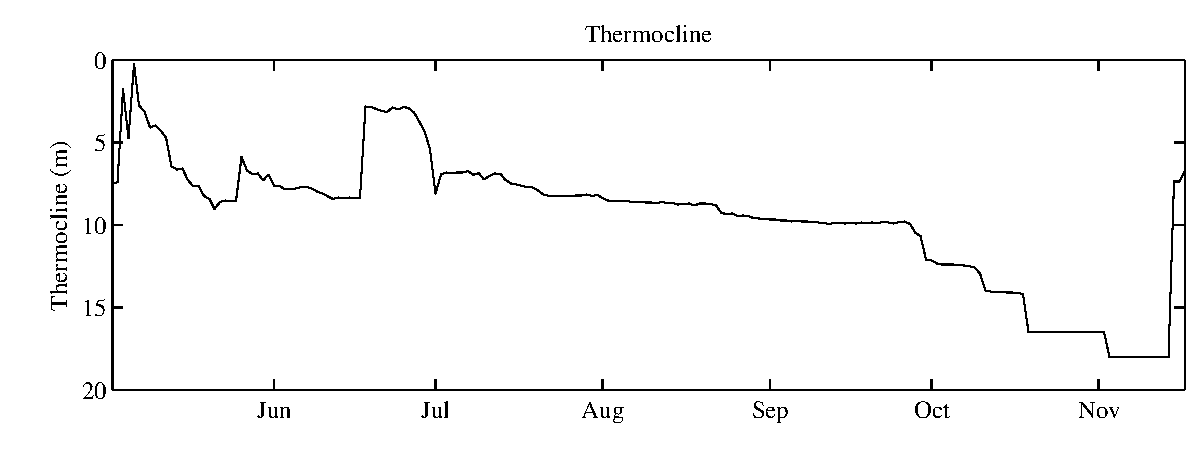
\includegraphics[width=.25\textwidth]{figures/Sparkling_thermD.pdf}}\\
    \subfigure{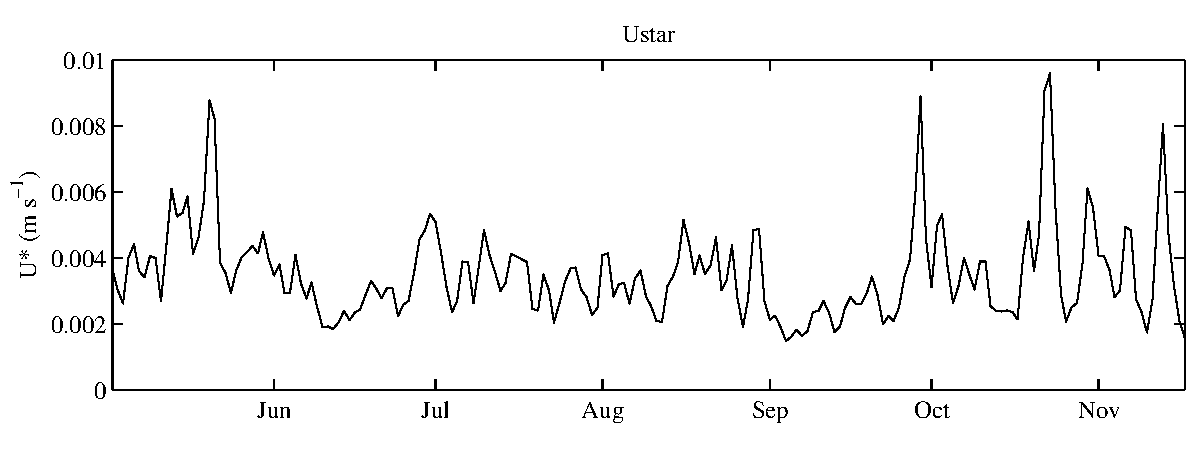
\includegraphics[width=.25\textwidth]{figures/Sparkling_uSt.pdf}}
    \subfigure{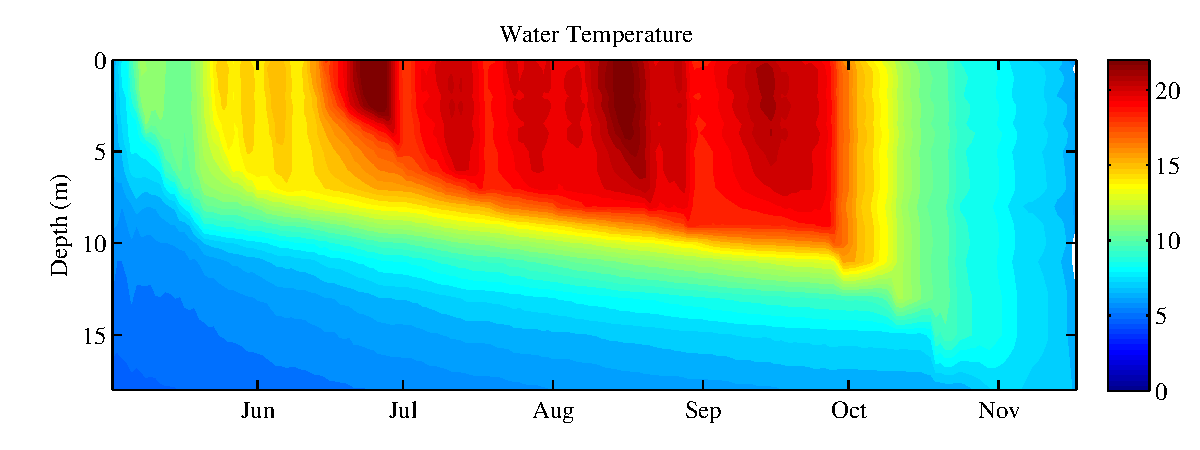
\includegraphics[width=.25\textwidth]{figures/Sparkling_wTemp.pdf}}
    \subfigure{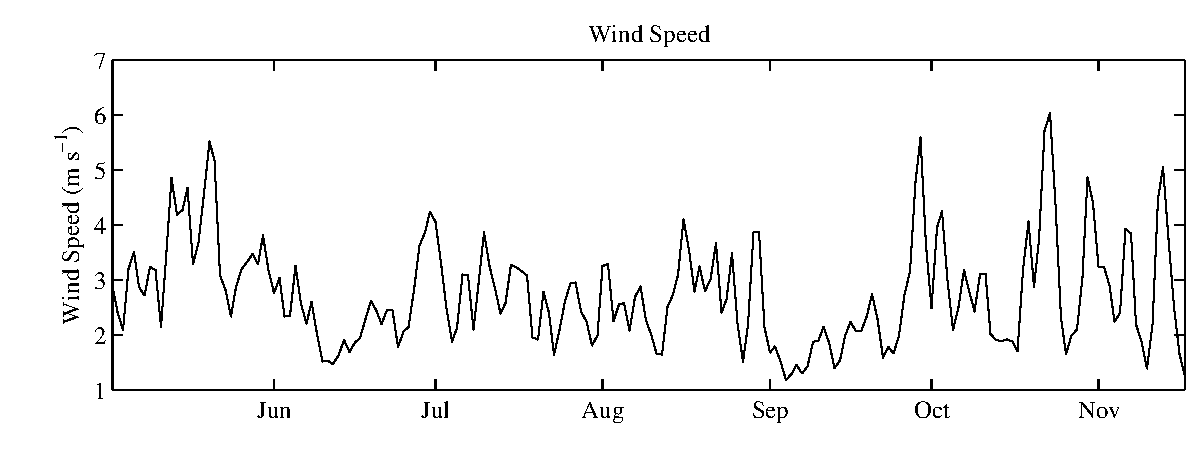
\includegraphics[width=.25\textwidth]{figures/Sparkling_wndSpd.pdf}}
  \end{figure}
\end{frame}

\titleframe{Streaming WPS}

\begin{frame}[t]{Streaming WPS}
  \begin{itemize}
    \item Allows streaming of of inputs and outputs to a WPS process
    \pause
    \item Previous approach:
    \begin{itemize}
      \item WPS is splitting inputs
      \item publishing results in a playlist that has to be checked constantly
    \end{itemize}
    \pause
    \item This approach:
    \begin{itemize}
      \item Sender splits inputs
      \item Sender starts a WPS streaming process
      \item Receiver connects to the WPS process
      \item Sender sends small chunks to the streaming process
      \item Streaming process pushes the results to the receiver
    \end{itemize}
  \end{itemize}
\end{frame}

\begin{frame}[t]{Streaming WPS}
  \begin{itemize}
    \item In a web-based (i.e. browser-based) environment, the WPS interface
    \begin{itemize}
      \item[\dots] does not allow subsequent inputs
      \item[\dots] does not allow intermediate outputs
    \end{itemize}
    \item Only possible with input/output references and long-lasting requests/polling
    \pause
    \item Solution: break out of the WPS interface
    \begin{itemize}
      \item Start a \emph{background} process
      \item Stream inputs/outputs using \emph{WebSockets}
    \end{itemize}
  \end{itemize}
\end{frame}

%\begin{frame}[t]{Streaming WPS --- Default Implementation}
%  \begin{itemize}
%    \item Single process
%    \pause
%    \item Delegate processing to a remote WPS process
%    \pause
%    \item Can turn any process into a streaming process
%    \pause
%    \item Can run forever
%  \end{itemize}
%\end{frame}

%\begin{frame}[c,fragile]{Streaming WPS --- Sequence Diagram}
  %\begin{figure}
    %\begin{center}
      %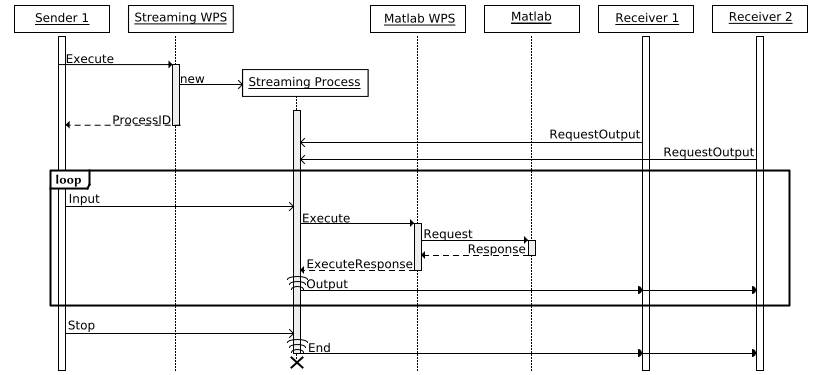
\includegraphics[width=\textwidth]{figures/sequence-diagram.pdf}
    %\end{center}
  %\end{figure}
%\end{frame}

\begin{frame}[c,fragile,label=sequencediagram]{Streaming WPS --- Sequence Diagram}
  \begin{figure}
    \begin{center}
      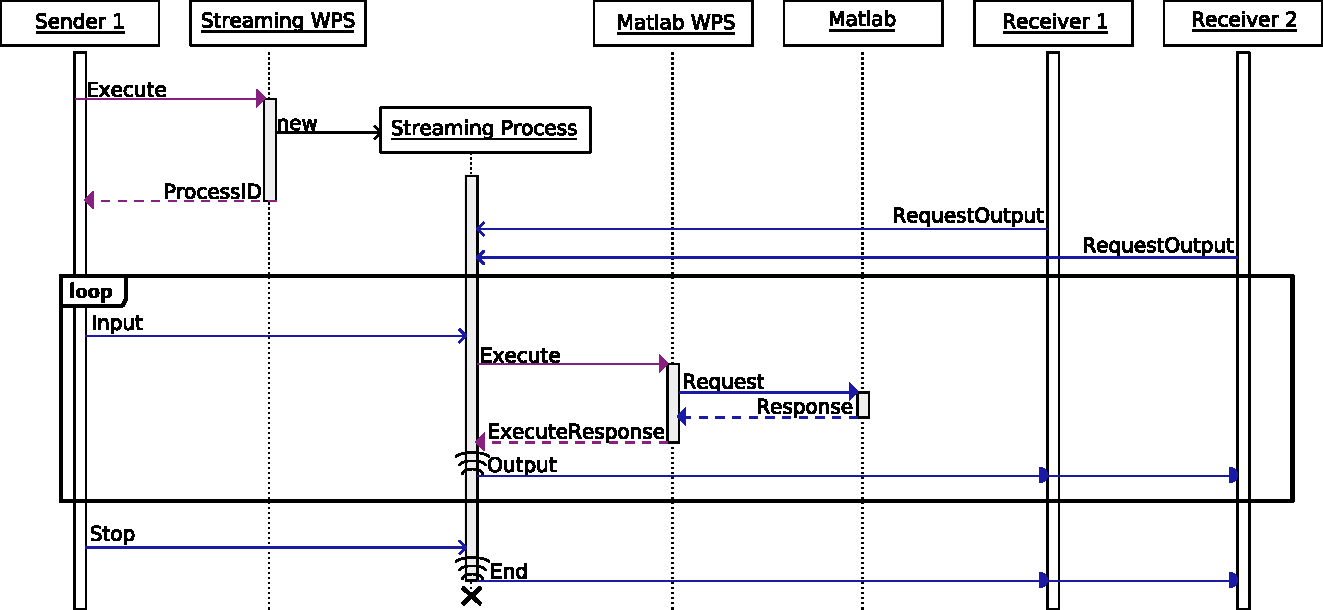
\includegraphics[width=\textwidth]{figures/sequence-diagram2.pdf}
    \end{center}
  \end{figure}
\end{frame}

\begin{frame}[c,fragile]{Streaming WPS --- Execute Request}
    \begin{center}
      \lstinputlisting[language=XML]{listings/streaming-execute.xml}
    \end{center}
\end{frame}

\begin{frame}[c,fragile]{Streaming WPS --- Execute Response}
    \begin{center}
      \lstinputlisting[language=XML]{listings/streaming-execute-response.xml}
    \end{center}
\end{frame}

\againframe{sequencediagram}

\begin{frame}[c,fragile]{Streaming WPS --- Output Request Message}
    \begin{center}
      \lstinputlisting[language=XML]{listings/streaming-output-request-message.xml}
    \end{center}
\end{frame}

\againframe{sequencediagram}

\begin{frame}[c,fragile]{Streaming WPS --- Input Message}
    \begin{center}
      \lstinputlisting[language=XML]{listings/streaming-input-message.xml}
    \end{center}
\end{frame}

\againframe{sequencediagram}

\begin{frame}[c,fragile]{Streaming WPS --- Output Message}
    \begin{center}
      \lstinputlisting[language=XML]{listings/streaming-output-message.xml}
    \end{center}
\end{frame}

\againframe{sequencediagram}

\begin{frame}[c,fragile]{Streaming WPS --- Stop Message}
    \begin{center}
      \lstinputlisting[language=XML]{listings/streaming-stop-message.xml}
    \end{center}
\end{frame}

\begin{frame}{Streaming WPS --- Input Types}
  \begin{itemize}
    \item Streaming Inputs
    \begin{itemize}
      \item submitted with \texttag{stream}{InputMessage}
      \item of type \texttag{wps}{Input}
    \end{itemize}
    \pause
    \item Static Inputs
    \begin{itemize}
      \item submitted with initial \texttag{wps}{Execute}
      \item merged with inputs of every streaming iteration
      \item of type \texttag{wps}{Input}
    \end{itemize}
    \pause
    \item Reference Inputs
    \begin{itemize}
      \item submitted with \texttag{stream}{InputMessage}
      \item references the output of a previous or upcoming streaming iteration
    \end{itemize}
    \pause
    \item Polling Inputs
  \end{itemize}
\end{frame}

\begin{frame}[t]{Streaming WPS --- Handling Dependencies}
  \begin{itemize}
    \item Clients declare dependencies to other streaming iterations (or their outputs)
    \item Automatic declaration of (spatial) dependencies not possibe as it is use case and format specific
    \item Process waits for all dependencies to become available
    \item Checking for cyclic dependencies/execution ordering
    \pause
    \begin{itemize}
      \arrow dynamic topological sort algorithm for directed acyclic graphs (based on breadth first search)
    \end{itemize}
  \end{itemize}
\end{frame}

\begin{frame}[c,fragile]{Streaming WPS --- Handling Dependencies}
  \begin{center}
    \lstinputlisting[language=XML,firstline=11,lastline=17]{listings/streaming-input-message.xml}
    \pause
    \lstinputlisting[language=XML,firstline=3,lastline=3]{listings/streaming-input-message.xml}
  \end{center}
\end{frame}

\titleframe{Current Status}

\begin{frame}[t]{Current Status}
  \begin{itemize}
    \item Done:
    \begin{itemize}
      \done Matlab WPS
      \done Lake Analyzer WPS
    \end{itemize}
    \pause
    \item WIP:
    \begin{itemize}
      \missing Streaming WPS
    \end{itemize}
    \pause
    \item Upcoming:
    \begin{itemize}
      \missing Webapp showcasing the process chain
    \end{itemize}
    \pause
    \item Sources:
    \begin{itemize}
      \arrow \url{https://github.com/autermann/Lake-Analyzer}
      \arrow \url{https://github.com/autermann/matlab-connector}
      \arrow \url{https://github.com/autermann/matlab-wps}
      \arrow \url{https://github.com/autermann/streaming-wps}
    \end{itemize}
  \end{itemize}
\end{frame}

\begin{frame}
  \vfill
  \begin{center}
    \emph{Thanks. Questions?}
  \end{center}
  \vfill
\end{frame}

\end{document}
